\chapter{排版软件及模板的使用方法}
公司在试用了多个排版软件之后,决定选用\LaTeX ,并使用统一的模板。\LaTeX 的工作方式为:用户编辑的文档为纯文本文件,配上用户需要的图片文件(或者原始数据文件),用 \LaTeX 软件处理成为 \filename{ps} 或 \filename{pdf} 文件。如图~\ref{latex} 所示。用户对版式的要求全部写在文本文件中,也就是用户需要了解一些\LaTeX 的排版语法。

\begin{figure}[htbp]\centering
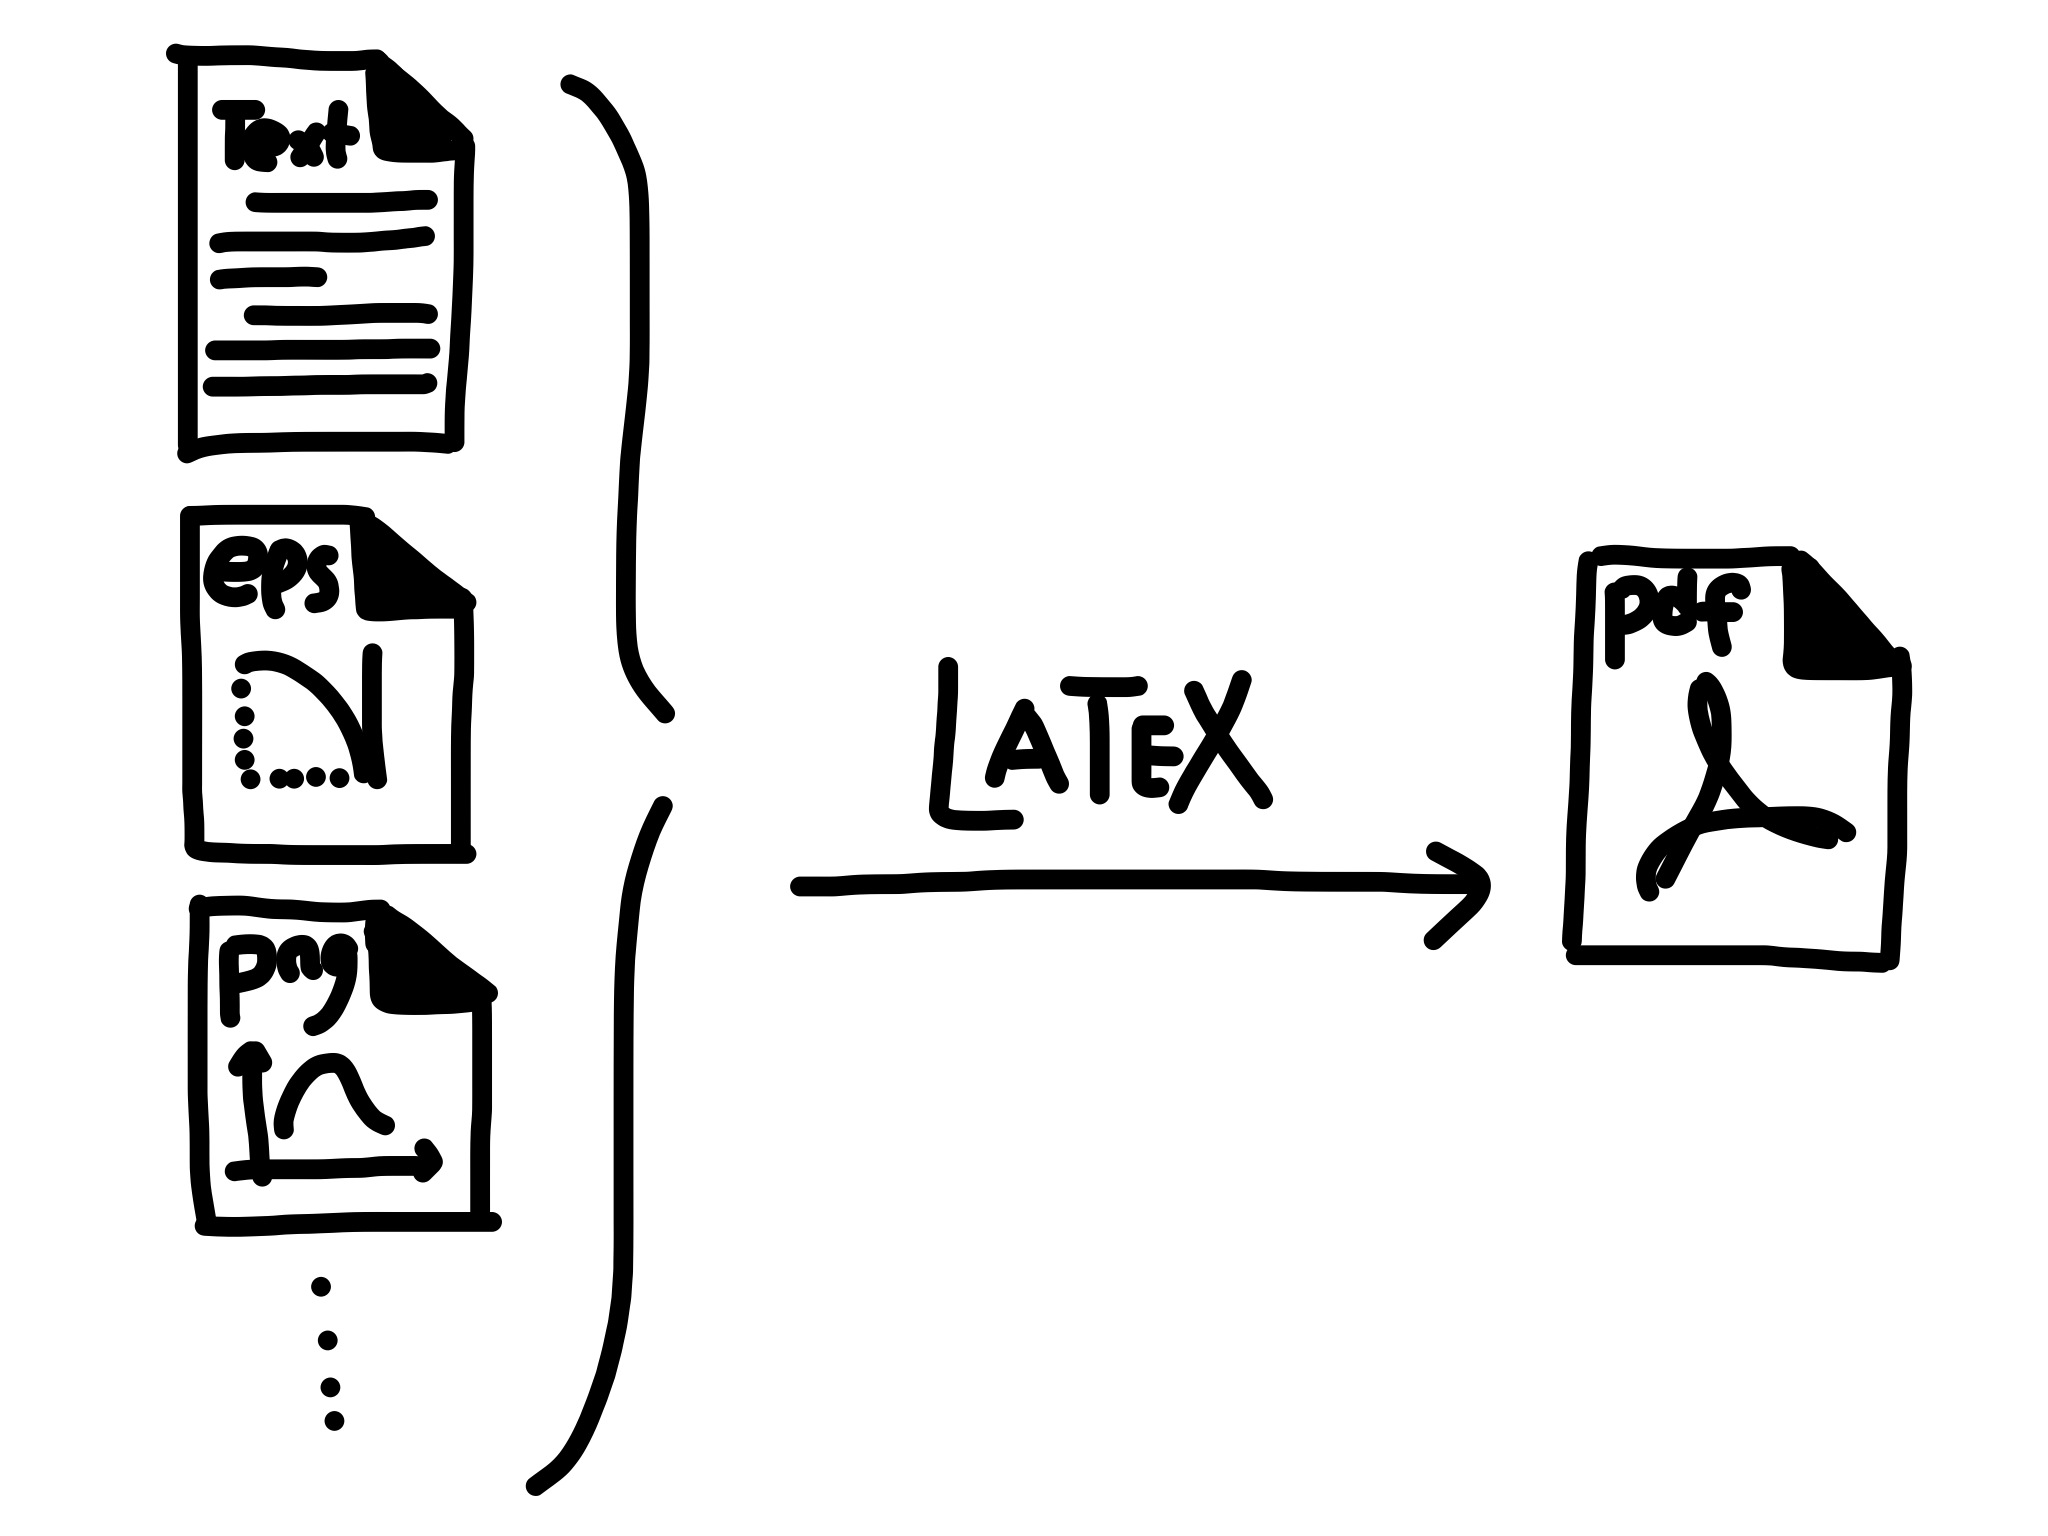
\includegraphics[width=0.45\textwidth]{latex_wm.jpg} 
\caption{\label{latex}\LaTeX 工作方式}
\end{figure}

公司选用\LaTeX 并采用统一的模板,好处为:
\begin{itemize}
\item 统一公司文档的风格。
\item 方便不同的人在不同平台下编辑和修改同一个文档。
\item 对于大型文档,\LaTeX 崩溃的概率小于其他常见排版软件;文本格式的文件损坏的概率也小。
\item \LaTeX 排出的版面更漂亮。
\item \LaTeX 免费。
\end{itemize}
坏处是用户编辑\TeX 文本文档时不够直观。对此公司的建议顺序是:
\begin{enumerate}
\item 使用纯文本编辑器编辑\TeX 文档,找一个\LaTeX 手册放在手边。(\LaTeX 常用的语法也就那么几页纸的事\cite{oetiker1995not}。)
\item 用 lyx 编辑。
\item 其他可输出\TeX 文档的软件。要求生成的\TeX 文档适于人工阅读。
\end{enumerate}

\section{软件的安装和使用}
目前我们公司使用的\LaTeX 发行包为 TexLive,你可以直接使用公司 Helium 服务器上的,也可以在自己的电脑上安装一份来用。以下分别介绍。

\subsection{在服务器上使用}
只需要设置使用 TexLive 软件所需的环境。
\begin{lstlisting}[language=sh,caption={在服务器上设置使用 TexLive 的环境}]
# Set the path environment of TexLive 
  source /usr/local/texlive/setenv.sh
# Or to make it permanent, you can simply do:
#    cat /usr/local/texlive/setenv.sh >> $HOME/.bash_profile
# test it
  which xelatex
\end{lstlisting}

\subsection{在自己电脑上安装}
目前我们使用的 TexLive 是个完整的庞大的包,其 \filename{iso} 镜像文件 2.4G,安装后需要 3.5G 的硬盘空间。安装前请在你自己的硬盘上准备充分的空间。
镜像文件为:\filename{/home/public/software /tex/texlive2013/texlive2013-*.iso}。
对于 Linux 系统,可能需要先几个字体文件。字体文件为 \filename{/home/public/sofware/tex/texlive2013/win\_fonts.tar.gz}。

假设你准备把字体安装在 \filename{/usr/share/fonts/TTF/}。安装方法为:
\begin{lstlisting}[language=sh,caption={安装字体}]
# copy the font files
  tar -xzvf win_fonts.tar.gz && sudo cp -r win_fonts /usr/share/fonts/TTF/
# activate the fonts
  sudo fc-chache -fv
\end{lstlisting}

假设你准备把 TexLive 安装在 \filename{/usr/local/tex} 。安装方法为:
\begin{lstlisting}[language=sh,caption={安装 TexLive}]
# mount the iso file
  sudo mount -o loop texlive2013-20130530.iso /mnt/dvd  && cd /mnt/dvd
# install it
  export TEXLIVE_INSTALL_PREFIX=/usr/local/tex
  perl install-tl
# then follow the instructions to set the path environment
  export PATH=/usr/local/texlive/2013/bin/x86_64-linux:$PATH
\end{lstlisting}

对于 Windows 用户,以上镜像文件也支持 Windows。请阅读镜像文件里的说明文件。

\subsection{Lyx}
Lyx 是一个直观的编辑\TeX 文件的编辑器。不需要 lyx 的人可以跳过这一节。服务器上已经安装了 lyx,你可以直接使用,也可以在自己电脑上安装。

在安装模板之前,需要先启动 lyx 一次以生成\filename{\$HOME/.lyx}。安装模板之后,启动 lyx 并点击\guimenu{Tools>{Reconfigure}},然后重新启动 lyx。

\section{模板的安装和使用}
公司的技术报告模板是放在用户自己目录下的,如此即使用户是在服务器上运行 TexLive,也需要安装模板。模板的路径:\filename{/home/public/document/template/cgdrep.tar.gz}。安装方法:
\begin{lstlisting}[language=sh,caption={安装模板}]
# Unpack the template
  tar xf /home/public/document/template/cgdrep.tar.gz
  cd cgdrep
# Install the template files
  ./install.sh
\end{lstlisting}

没有报错的话,可以使用 \LaTeX 模板的示例了:
\begin{lstlisting}[language=sh,caption={模板示例}]
# test the LaTeX example
  cd example/latex
  make
# There should be several new files and one of them is main.pdf
  evince main.pdf &
\end{lstlisting}
